\begin{aosachapter}{Audacity}{s:audacity}{James Crook}

Audacity is a popular sound recorder and audio editor.  It is a
capable program while still being easy to use.  The majority of users
are on Windows but the same Audacity source code compiles to run on
Linux and Mac too.

Dominic Mazzoni wrote the original version of Audacity in 1999 while
he was a research student at Carnegie Mellon University.  Dominic
wanted to create a platform on which to develop and debug audio
processing algorithms.  The software grew to become useful in its own
right in many other ways.  Once Audacity was released as open source
software, it attracted other developers.  A small, gradually-changing
team of enthusiasts have modified, maintained, tested, updated,
written documentation for, helped users with, and translated
Audacity's interface into other languages over the years.

One goal is that its user interface should be discoverable:
people should be able to sit down without a manual and start using it
right away, gradually discovering its features.  This principle has
been crucial in giving Audacity greater consistency to the user
interface than there otherwise would be.  For a project in which many
people have a hand this kind of unifying principle is more important
than it might seem at first.

It would be good if the architecture of Audacity had a similar guiding
principle, a similar kind of discoverability.  The closest we have to
that is ``try and be consistent''.  When adding new code, developers try
to follow the style and conventions of code nearby.  In practice,
though, the Audacity code base is a mix of well-structured and less
well-structured code.  Rather than an overall architecture the analogy
of a small city is better: there are some impressive buildings but you
will also find run-down neighborhoods that are more like a shanty
town.

\begin{aosasect1}{Structure in Audacity}

Audacity is layered upon several libraries.  While most new
programming in Audacity code doesn't require a detailed knowledge of
exactly what is going on in these libraries, familiarity with their
APIs and what they do is important.  The two most important libraries
are PortAudio which provides a low-level audio interface in a
cross-platform way, and wxWidgets which provides GUI components in a
cross-platform way.

When reading Audacity's code,
it helps to realize that only a fraction of the code is essential.
Libraries contribute a lot of optional features---though people who
use those features might not consider them optional.  For example, as
well as having its own built-in audio effects, Audacity supports
LADSPA (Linux Audio Developer's Simple Plugin API) for dynamically
loadable plugin audio effects.  The VAMP API in Audacity does the same
thing for plugins that analyze audio.  Without these APIs, Audacity
would be less feature-rich, but it does not absolutely depend on these
features.

Other optional libraries used by Audacity are libFLAC, libogg,
and libvorbis.  These provide various audio compression formats.  MP3
format is catered for by dynamically loading the LAME or FFmpeg
library.  Licensing restrictions prevent these very popular
compression libraries from being built-in.

Licensing is behind some other decisions about Audacity libraries and
structure.  For example, support for VST plugins
is not built in because of licensing restrictions.
We would also like to use the very efficient FFTW
fast Fourier transform code in some of our code.  However, we only
provide that as an option for people who compile Audacity themselves,
and instead fall back to a slightly slower version in our normal
builds.  As long as Audacity accepts plugins, it can be and has been
argued that Audacity cannot use FFTW\@.  FFTW's authors do not want
their code to be available as a general service to arbitrary other
code.  So, the architectural decision to support plugins leads to a
trade-off in what we can offer.  It makes LADSPA plugins possible but
bars us from using FFTW in our pre-built executables.

Architecture is also shaped by considerations of how best to use our
scarce developer time.  With a small team of developers, we do not
have the resources to do, for example, the in-depth analysis of
security loopholes that teams working on Firefox and Thunderbird do.
However, we do not want Audacity to provide a route to bypass a
firewall, so we have a rule not to have TCP/IP connections to or from
Audacity at all.  Avoiding TCP/IP cuts out many security concerns.
The awareness of our limited resources leads us to better design.  
It helps us cut features that would cost us too much in developer 
time and focus on what is essential.

A similar concern for developers' time applies to scripting languages.
We want scripting, but the code implementing the languages does not
need to be in Audacity.  It does not make sense to compile copies of
each scripting language into Audacity to give users all the choices
they could want.\footnote{The one exception to this is the Lisp-based
Nyquist language which has been built into Audacity from very early
days.  We would like to make it a separate module, bundled with
Audacity, but we have not yet had the time to make that change.}
We have instead implemented scripting with a single plugin module and a
pipe, which we will cover later.

\aosafigure[350pt]{../images/audacity/Layers.png}{Layers in Audacity}{fig.aud.1}

\aosafigref{fig.aud.1} shows some layers and modules in Audacity.  The
diagram highlights three important classes within wxWidgets, each of
which has a reflection in Audacity.  We're building higher-level
abstractions from related lower-level ones.  For example, the
BlockFile system is a reflection of and is built on wxWidgets'
wxFiles.  It might, at some stage, make sense to split out BlockFiles,
ShuttleGUI, and command handling into an intermediate library in their
own right.  This would encourage us to make them more general.

Lower down in the diagram is a narrow strip for ``Platform Specific
Implementation Layers.'' Both wxWidgets and PortAudio are OS
abstraction layers.  Both contain conditional code that chooses
between different implementations depending on the target platform.

The ``Other Supporting Libraries'' category includes a wide collection
of libraries.  Interestingly quite a few of these rely on dynamically
loaded modules.  Those dynamic modules know nothing of wxWidgets.

On the Windows platform we used to compile Audacity as a single
monolithic executable with wxWidgets and Audacity application code in
the same executable.  In 2008 we changed over to using a modular
structure with wxWidgets as a separate DLL\@.  This is to allow
additional optional DLLs to be loaded at run time where those DLLs
directly use features of wxWidgets.  Plugins that plug in above the
dotted line in the diagram can use wxWidgets.

The decision to use DLLs for wxWidgets has its downsides.  The
distribution is now larger, partly because many unused functions are
provided in the DLLs that would previously have been optimized away.
Audacity also takes longer to start up because each DLL is loaded
separately.  The advantages are considerable.  We expect modules
to have similar advantages for us as they do for Apache.  As we see
it, modules allow the core of Apache to be very stable while
facilitating experimentation, special features and new ideas in the
modules.  Modules go a very long way to counteracting the temptation
to fork a project to take it in a new direction.  We think it's been a
very important architectural change for us.  We're expecting these
advantages but have not seen them yet.  Exposing the wxWidgets
functions is only a first step and we have more to do to have a
flexible modular system.

The structure of a program like Audacity clearly is not designed up
front.  It is something that develops over time.  By and large the
architecture we now have works well for us.  We find ourselves
fighting the architecture when we try to add features that affect many
of the source files.  For example, Audacity currently handles stereo
and mono tracks in a special cased way.  If you wanted to modify
Audacity to handle surround sound you'd need to make changes in many
classes in Audacity.
\newpage %to keep this sidebar right here.
\begin{aosabox}{Going Beyond Stereo: The \code{GetLink} Story}

Audacity has never had an abstraction for number of channels.  Instead
the abstraction it uses is to link audio channels.  There is a
function \code{GetLink}that returns the other audio channel in a pair
if there are two and that returns NULL if the track is mono.  Code
that uses \code{GetLink} typically looks exactly as if it were
originally written for mono and later a test of \code{(GetLink() !=
  NULL)} used to extend that code to handle stereo.  I'm not sure it
was actually written that way, but I suspect it.  There's no looping
using \code{GetLink} to iterate through all channels in a linked list.
Drawing, mixing, reading and writing all contain a test for the stereo
case rather than general code that can work for n channels where n is
most likely to be one or two.  To go for the more general code you'd
need to make changes at around 100 of these calls to the
\code{GetLink} function modifying at least 26 files.

It's easy to search the code to find \code{GetLink} calls and the
changes needed are not that complex, so it is not as big a deal to fix
this ``problem'' as it might sound at first.  The \code{GetLink} story
is not about a structural defect that is hard to fix.  Rather it's
illustrative of how a relatively small defect can travel into a lot of
code, if allowed to.

With hindsight it would have been good to make the \code{GetLink}
function private and instead provide an iterator to iterate through
all channels in a track.  This would have avoided much special case code for
stereo, and at the same time made code that uses the
list of audio channels agnostic with respect to the list implementation.

\end{aosabox}

The more modular design is likely to drive us towards better hiding of
internal structure.  As we define and extend an external API we'll
need to look more closely at the functions we're providing.  This will
draw our attention to abstractions that we don't want to lock in to an
external API.

\end{aosasect1}

\begin{aosasect1}{wxWidgets GUI Library}

The most significant single library for Audacity user interface
programmers is the wxWidgets GUI library, which provides such
things as buttons, sliders, check boxes, windows and dialogs.  It provides
the most visible cross-platform behavior.  The wxWidgets library has
its own string class \code{wxString}, it has cross-platform
abstractions for threads, filesystems, and fonts, and a mechanism for
localization to other languages, all of which we use.  We advise
people new to Audacity development to first download wxWidgets and
compile and experiment with some of the samples that come with that
library.  wxWidgets is a relatively thin layer on the underlying GUI
objects provided by the operating system.

To build up complex dialogs wxWidgets provides not only individual
widget elements but also sizers that control the elements' sizes
and positions.  This is a lot nicer than giving absolute fixed
positions to graphical elements.  If the widgets are resized either
directly by the user or, say, by using a different font size, the
positioning of the elements in the dialogs updates in a very natural
way.  Sizers are important for a cross-platform application.  Without
them we might have to have custom layouts of dialogs for each
platform.

Often the design for these dialogs is in a resource file that is
read by the program.  However in Audacity we exclusively compile
dialog designs into the program as a series of calls to wxWidgets
functions.  This provides maximum flexibility: that is, dialogs whose
exact contents and behavior will be determined by application level
code.

You could at one time find places in Audacity where the initial code
for creating a GUI had clearly been code-generated using a graphical
dialog building tool.  Those tools helped us get a basic design.  Over
time the basic code was hacked around to add new features,
resulting in many places where new dialogs were created by
copying and modifying existing, already hacked-around
dialog code.

After a number of years of such development we found that large
sections of the Audacity source code, particularly the dialogs for
configuring user preferences, consisted of tangled repetitive code.
That code, though simple in what it did, was surprisingly hard to
follow.  Part of the problem was that the sequence in which dialogs
were built up was quite arbitrary: smaller elements were combined into
larger ones and eventually into complete dialogs, but the order in
which elements were created by the code did not (and did not need to)
resemble the order elements were laid out on screen.  The code was
also verbose and repetitive.  There was GUI-related code to transfer
data from preferences stored on disk to intermediate variables, code
to transfer from intermediate variables to the displayed GUI, code to
transfer from the displayed GUI to intermediate variables, and code to
transfer from intermediate variables to the stored preferences.  There
were comments in the code along the lines of \code{//this is a mess},
but it was quite some time before anything was done about it.

\end{aosasect1}

\begin{aosasect1}{ShuttleGui Layer}

The solution to untangling all this code was a new class, ShuttleGui,
that much reduced the number of lines of code needed to specify a
dialog, making the code more readable.  ShuttleGui is an extra layer
between the wxWidgets library and Audacity.  Its job is to transfer
information between the two.  Here's an example which results in the
GUI elements pictured in \aosafigref{fig.aud.2}.

\begin{figure}[h!]
\begin{minipage}[b]{7cm}
\begin{verbatim}
ShuttleGui S;
// GUI Structure
S.StartStatic("Some Title",...);
{
    S.AddButton("Some Button",...);
    S.TieCheckbox("Some Checkbox",...);
}
S.EndStatic();
\end{verbatim}
\end{minipage}
\begin{minipage}[b]{7cm}
% \aosafigure[200pt]{../images/audacity/SomeDialog.png}{Example Dialog}{fig.aud.2}
\centering
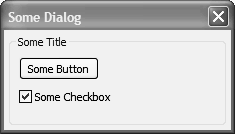
\includegraphics[width={150pt}]{../images/audacity/SomeDialog.png}
\end{minipage}
\caption{Example Dialog}
\label{fig.aud.2}
\end{figure}

This code defines a static box in a dialog and that box contains a
button and a checkbox.  The correspondence between the code and the
dialog should be clear.  The \code{StartStatic} and \code{EndStatic}
are paired calls.  Other similar
\code{StartSomething}/\code{EndSomething} pairs, which must match, are
used for controlling other aspects of layout of the dialog.  The curly
brackets and the indenting that goes with them aren't needed for this
to be correct code.  We adopted the convention of adding them in to
make the structure and particularly the matching of the paired calls
obvious.  It really helps readability in larger examples.

The source code shown does not just create the dialog.  The code after
the comment ``\code{//GUI Structure}'' can also be used to shuttle
data from the dialog out to where the user preferences are stored, and
to shuttle data back in.  Previously a lot of the repetitive code came
from the need to do this.  Nowadays that code is only written once and
is buried within the \code{ShuttleGui} class.

There are other extensions to the basic wxWidgets in Audacity.
Audacity has its own class for managing toolbars.  Why doesn't it use
wxWidget's built in toolbar class?  The reason is historic: Audacity's
toolbars were written before wxWidgets provided a toolbar class.

\end{aosasect1}

\begin{aosasect1}{The TrackPanel}

The main panel in Audacity which displays audio waveforms is the
TrackPanel.  This is a custom control drawn by Audacity.  It's made up
of components such as smaller panels with track information, a ruler
for the timebase, rulers for amplitude, and tracks which may show
waveforms, spectra or textual labels.  The tracks can be resized and
moved around by dragging.  The tracks containing textual labels make
use of our own re-implementation of an editable text box rather than
using the built-in text box.  You might think these panels tracks and
rulers should each be a wxWidgets component, but they are not.

\aosafigure{../images/audacity/MainPanelAnnotated.png}{Audacity Interface with Track Panel Elements Labelled}{fig.aud.3}

The screenshot shown in \aosafigref{fig.aud.3} shows the Audacity user
interface.  All the components that have been labelled are custom for
Audacity.  As far as wxWidgets is concerned there is one wxWidget
component for the TrackPanel.  Audacity code, not wxWidgets, takes
care of the positioning and repainting within that.

The way all these components fit together to make the TrackPanel is
truly horrible.  (It's the code that's horrible; the end result the
user sees looks just fine.)  The GUI and application-specific code is
all mixed together, not separated cleanly.  In a good design only our
application-specific code should know about left and right audio
channels, decibels, muting and soloing.  GUI elements should be
application agnostic elements that are reusable in a non-audio
application.  Even the purely GUI parts of TrackPanel are a patchwork
of special case code with absolute positions and sizes and not enough
abstraction.  It would be so much nicer, cleaner and more consistent
if these special components were self-contained GUI elements and if
they used sizers with the same kinds of interface as wxWidgets uses.

To get to such a TrackPanel we'd need a new sizer for wxWidgets that
can move and resize tracks or, indeed, any other widget.  wxWidgets
sizers aren't yet that flexible.  As a spin off benefit we could use
that sizer elsewhere.  We could use it in the toolbars that hold the
buttons, making it easy to customize the order of buttons within a
toolbar by dragging.

Some exploratory work has been done in creating and using such sizers,
but not enough.  Some experiments with making the GUI components fully
fledged wxWidgets ran into a problem: doing so reduces our control
over repainting of the widgets, resulting in flicker when resizing and
moving components.  We would need to
extensively modify wxWidgets to achieve flicker-free repainting, and
better separate the resizing steps from the repainting steps.

A second reason to be wary of this approach for the TrackPanel is that
we already know wxWidgets start running very slowly when there are
large numbers of widgets.  This is mostly outside of wxWidget's
control.  Each wxWidget, button, and text entry box uses a
resource from the windowing system. Each has a handle to access it.
Processing large numbers of these takes time.  Processing is slow even
when the majority of widgets are hidden or off screen.  We want to be
able to use many small widgets on our tracks.

The best solution is to use a flyweight pattern, lightweight
widgets that we draw ourselves, which do not have corresponding
objects that consume windowing system resources or handles.  We would
use a structure like wxWidgets's sizers and component widgets, and
give the components a similar API but not actually derive from
wxWidgets classes.  We'd be refactoring our existing TrackPanel code
so that its structure became a lot clearer.  If this were an easy
solution it would already have been done, but diverging opinions about
exactly what we want to end up with derailed an earlier attempt.
Generalizing our current ad hoc approach would take significant design
work and coding.  There is a great temptation to leave complex code
that already works well enough alone.

\end{aosasect1}

\begin{aosasect1}{PortAudio Library: Recording and Playback}

PortAudio is the audio library that gives Audacity the ability to play
and record audio in a cross-platform way.  Without it Audacity would
not be able to use the sound card of the device it's running on.
PortAudio provides the ring
buffers, sample rate conversion when playing/recording and, crucially,
provides an API that hides the differences between audio on Mac, Linux
and Windows.  Within PortAudio there are alternative implementation
files to support this API for each platform.

I've never needed to dig into PortAudio to follow what happens inside.
It is, however, useful to know how we interface with PortAudio.
Audacity accepts data packets from PortAudio (recording) and sends
packets to PortAudio (playback).  It's worth looking at
exactly how the sending and
receiving happens, and how it fits in with reading and writing to disk
and updates to the screen.

Several different processes are going on at the same time.  Some
happen frequently, transfer small amounts of data, and must be
responded to quickly.  Others happen less frequently, transfer larger
quantities of data, and the exact timing of when they happen is less
critical.  This is an impedance mismatch between the processes,
and buffers are used to accommodate it.  A second part of the picture is
that we are dealing with audio devices, hard drives,
and the screen.  We don't go down to the wire and so have to work with
the APIs we're given.  Whilst we would like each of our processes to
look similar, for example to have each running from a wxThread, we
don't have that luxury (\aosafigref{fig.aud.4}).

\aosafigureTop[325pt]{../images/audacity/Buffers.png}{Threads and Buffers in Playback and Recording}{fig.aud.4}

One audio thread is started by PortAudio code and interacts directly
with the audio device.  This is what drives recording or playback.
This thread has to be responsive or packets will get lost.  The
thread, under the control of PortAudio code, calls
\code{audacityAudioCallback} which, when recording, adds newly arrived
small packets to a larger (five second) capture buffer.  When playing
back it takes small chunks off a five second playback buffer.  The
PortAudio library knows nothing about wxWidgets and so this thread
created by PortAudio is a pthread.

A second thread is started by code in Audacity's class AudioIO\@.  When
recording, AudioIO takes the data from the capture buffer and appends
it to Audacity's tracks so that it will eventually get displayed.
Additionally, when enough data has been added, AudioIO writes the data
to disk.  This same thread also does the disk reads for audio
playback.  The function \code{AudioIO::FillBuffers} is the key
function here and depending on the settings of some Boolean variables,
handles both recording and playback in the one function.  It's
important that the one function handle both directions.  Both the
recording and playback parts are used at the same time when doing
``software play through,'' where you overdub what was previously
recorded.  In the AudioIO thread we are totally at the mercy of the
operating system's disk IO\@.  We may stall for an unknown length of
time reading or writing to a disk.  We could not do those reads or
writes in \code{audacityAudioCallback} because of the need to be
responsive there.

Communication between these two threads happens via shared variables.
Because we control which threads are writing to these variables and
when, we avoid the need for more expensive mutexes.

\pagebreak

In both playback and recording, there is an additional requirement:
Audacity also needs to update the GUI\@.  This is the least time
critical operation.  The update happens in the main GUI thread and is
due to a periodic timer that ticks twenty times a second.  This
timer's tick causes \code{TrackPanel::OnTimer} to be called, and if
updates to the GUI are found to be needed, they are applied.  This
main GUI thread is created within wxWidgets rather than by our own
code.  It is special in that other threads cannot directly update the
GUI\@.  Using a timer to get the GUI thread to check if it needs to
update the screen allows us to reduce the number of repaints to a
level that is acceptable for a responsive display, and not make too
heavy demands on processor time for displaying.

Is it good design to have an audio device thread, a buffer/disk thread
and a GUI thread with periodic timer to handle these audio data
transfers?  It is somewhat ad hoc to have these three different
threads that are not based on a single abstract base class.  However,
the ad-hockery is largely dictated by the libraries we use.  PortAudio
expects to create a thread itself.  The wxWidgets framework
automatically has a GUI thread.  Our need for a buffer filling thread
is dictated by our need to fix the impedance mismatch between the
frequent small packets of the audio device thread and the less
frequent larger packets of the disk drive.  There is very clear
benefit in using these libraries.  The cost in using the libraries is
that we end up using the abstractions they provide.  As a result we
copy data in memory from one place to another more than is strictly
necessary.  In fast data switches I've worked on, I've seen extremely
efficient code for handling these kinds of impedance mismatches
that is interrupt driven and does not use threads at all.  Pointers to
buffers are passed around rather than copying data.  You can only do
that if the libraries you are using are designed with a richer buffer
abstraction.  Using the existing interfaces, we're forced to use
threads and we're forced to copy data.

\end{aosasect1}

\begin{aosasect1}{BlockFiles}

One of the challenges faced by Audacity is supporting insertions and
deletions into audio recordings that may be hours long.  Recordings
can easily be too long to fit in available RAM\@.  If an audio recording
is in a single disk file, inserting audio somewhere near the start of
that file could mean moving a lot of data to make way.  Copying that
data on disk would be time consuming and mean that Audacity could then
not respond rapidly to simple edits.

Audacity's solution to this is to divide audio files into many
BlockFiles, each of which could be around 1 MB\@.  This is the main
reason Audacity has its own audio file format, a master file with the
extension \code{.aup}.  It is an XML file which coordinates the various
blocks.  Changes near the start of a long audio recording might affect
just one block and the master \code{.aup} file.

BlockFiles balance two conflicting forces.  We can insert and delete
audio without excessive copying, and during playback we are guaranteed
to get reasonably large chunks of audio with each request to the disk.
The smaller the blocks, the more potential disk requests to fetch the
same amount of audio data; the larger the blocks, the more copying on
insertions and deletions.

Audacity's BlockFiles never have internal free space and they never
grow beyond the maximum block size.  To keep this true when we insert
or delete we may end up copying up to one block's worth of data.  When
we don't need a BlockFile anymore we delete it.  The BlockFiles are
reference counted so if we delete some audio, the relevant BlockFiles
will still hang around to support the undo mechanism until we save.
There is never a need to garbage collect free space within
Audacity BlockFiles, which we would need to do with an all-in-one-file
approach.

Merging and splitting larger chunks of data is the bread and butter of
data management systems, from B-trees to Google's BigTable tablets to
the management of unrolled linked lists.  \aosafigref{fig.aud.5} shows
what happens in Audacity when removing a span of audio near the start.

\aosafigure[200pt]{../images/audacity/BlocksCombined.png}{Before deletion, \code{.aup} file and BlockFiles hold the sequence ABCDEFGHIJKLMNO. After deletion of FGHI, two BlockFiles are merged.}{fig.aud.5}

BlockFiles aren't just used for the audio itself.  There are also
BlockFiles that cache summary information.  If Audacity is asked to
display a four hour long recording on screen it is not acceptable for
it to process the entire audio each time it redraws the screen.
Instead it uses summary information which gives the maximum and
minimum audio amplitude over ranges of time.  When zoomed in,
Audacity is drawing using actual samples.  When zoomed out,
Audacity is drawing using summary information.

A refinement in the BlockFile system is that the blocks needn't be
files created by Audacity.  They can be references to subsections of
audio files such as a timespan from audio stored in the \code{.wav} format.
A user can create an Audacity project, import audio from a \code{.wav} file
and mix a number of tracks whilst only creating BlockFiles for the
summary information.  This saves disk space and saves time in copying
audio.  All told it is, however, a rather bad idea.  Far too many of
our users have removed the original audio \code{.wav} file thinking there
will be a complete copy in the Audacity project folder.  That's not so
and without the original \code{.wav} file the audio project can no longer be
played.  The default in Audacity nowadays is to always copy imported
audio, creating new BlockFiles in the process.

The BlockFile solution ran into problems on Windows systems where
having a large number of BlockFiles performed very poorly.  This appeared
to be because Windows was much slower handling
files when there were many in the same directory, a similar problem to
the slowdown with large numbers of widgets.  A later addition was made
to use a hierarchy of subdirectories, never with more than a hundred
files in each subdirectory.

The main problem with the BlockFile structure is that it is exposed to
end users.  We often hear from users who move the \code{.aup} file and don't
realize they also need to move the folder containing all the
BlockFiles too.  It would be better if Audacity projects were a single
file with Audacity taking responsibility for how the space inside the
file is used.  If anything this would increase performance rather than
reduce it.  The main additional code needed would be for garbage
collection.  A simple approach to that would be to copy the blocks to
a new file when saving if more than a set percentage of the file were
unused.

\end{aosasect1}

\begin{aosasect1}{Scripting}

Audacity has an experimental plugin that supports multiple scripting
languages.  It provides a scripting interface over a named pipe.  The
commands exposed via scripting are in a textual format, as are the
responses.  As long as the user's scripting language can write text to
and read text from a named pipe, the scripting language can drive
Audacity.  Audio and other high-volume data does not need to travel on
the pipe (\aosafigref{fig.aud.7}).

\aosafigure[75pt]{../images/audacity/Scripting.png}{Scripting Plugin Provides Scripting Over a Named Pipe}{fig.aud.7}

The plugin itself knows nothing about the content of the text traffic
that it carries. It is only responsible for conveying it. The plugin
interface (or rudimentary extension point) used by the scripting
plugin to plug in to Audacity already exposes Audacity commands in
textual format.  So, the scripting plugin is small, its main content
being code for the pipe.

Unfortunately a pipe introduces similar security risks to having a
TCP/IP connection---and we've ruled out TCP/IP connections for
Audacity on security grounds.  To reduce that risk the plugin is an
optional DLL\@.  You have to make a deliberate decision to obtain and
use it and it comes with a health/security warning.

After the scripting feature had already been started, a suggestion
surfaced in the feature requests page of our wiki that we should
consider using KDE's D-Bus standard to provide an inter-process call
mechanism using TCP/IP\@.  We'd already started going down a different
route but it still might make sense to adapt the interface we've ended
up with to support D-Bus.

\begin{aosabox}{Origins of Scripting Code}

The scripting feature grew from an enthusiast's adaptation of Audacity
for a particular need that was heading in the direction of being a
fork.  These features, together called CleanSpeech, provide for mp3
conversion of sermons.  CleanSpeech adds new effects such as truncate
silence---the effect finds and cuts out long silences in audio---and
the ability to apply a fixed sequence of existing noise removal
effects, normalization and mp3 conversion to a whole batch of audio
recordings.  We wanted some of the excellent functionality in this,
but the way it was written was too special case for Audacity.
Bringing it into mainstream Audacity led us to code for a flexible
sequence rather than a fixed sequence.  The flexible sequence could
use any of the effects via a look-up table for command names and a
\code{Shuttle} class to persist the command parameters to a textual
format in user preferences.  This feature is called \emph{batch
chains}.  Very deliberately we stopped short of adding conditionals
or calculation to avoid inventing an ad hoc scripting language.

In retrospect the effort to avoid a fork has been well worthwhile.
There is still a CleanSpeech mode buried in Audacity that can be
set by modifying a preference. It also cuts down the user interface,
removing advanced features. A simplified version of Audacity has been
requested for other uses, most notably in schools. The problem is that
each person's view of which are the advanced features and which are
the essential ones is different.  We've subsequently implemented a
simple hack that leverages the translation mechanism.  When the
translation of a menu item starts with a ``\#'' it is no longer shown
in the menus.  That way people who want to reduce the menus can make
choices themselves without recompiling---more general and less
invasive than the \code{mCleanspeech} flag in Audacity, which in time we
may be able to remove entirely.

The CleanSpeech work gave us batch chains and the ability to
truncate silence.  Both
have attracted additional improvement from outside the core team.
Batch chains directly led on to the scripting feature.  That in turn
has begun the process of supporting more general purpose plugins to
adapt Audacity.

\end{aosabox}

\end{aosasect1}

\begin{aosasect1}{Real-Time Effects}

Audacity does not have real-time effects, that is, audio effects that
are calculated on demand as the audio plays.  Instead in Audacity you
apply an effect and must wait for it to complete.  Real-time effects
and rendering of audio effects in the background whilst the user
interface stays responsive are among the most frequently made
feature requests for Audacity.

A problem we have is that what may be a real-time effect on one
machine may not run fast enough to be real-time on a much slower
machine.  Audacity runs on a wide range of machines.  We'd like a
graceful fallback.  On a slower machine we'd still want to be able to
request an effect be applied to an entire track and to then listen to
the processed audio near the middle of the track, after a small wait,
with Audacity knowing to process that part first.  On a machine too
slow to render the effect in real time we'd be able to listen to the
audio until playback caught up with the rendering.  To do this we'd
need to remove the restrictions that audio effects hold up the user
interface and that the order of processing the audio blocks is
strictly left to right.

A relatively recent addition in Audacity called \emph{on demand loading}
has many of the elements we need for real time effects, though it
doesn't involve audio effects at all.  When you import an audio file
into Audacity, it can now make the summary BlockFiles in a background
task.  Audacity will show a placeholder of diagonal blue and gray
stripes for audio that it has not yet processed and respond to many
user commands whilst the audio is still being loaded.  The blocks do
not have to be processed in left-to-right order.  The intention has
always been that the same code will in due course be used for
real-time effects.

On demand loading gives us an evolutionary approach to adding real
time effects.  It's a step that avoids some of the complexities of
making the effects themselves real-time.  Real-time effects will
additionally need overlap between the blocks, otherwise effects like
echo will not join up correctly.  We'll also need to allow parameters
to vary as the audio is playing.  By doing on demand loading first,
the code gets used at an earlier stage than it otherwise would.  It
will get feedback and refinement from actual use.

\end{aosasect1}

\begin{aosasect1}{Summary}

The earlier sections of this chapter illustrate how good structure
contribute to a program's growth, or how the absence of good structure
hinders it.

\begin{aosaitemize}

\item Third party APIs such as PortAudio and wxWidgets have been of
  huge benefit.  They've given us code that works to build on, and
  abstracted away many platform differences.  One price we pay for
  using them is that we don't get the flexibility to choose the
  abstractions.  We have less than pretty code for playback and
  recording because we have to handle threading in three different
  ways.  The code also does more copying of data than it could do if
  we controlled the abstractions.

\item The API given to us by wxWidgets tempted us into writing some
  verbose, hard to follow application code.  Our solution to that was
  to add a facade in front of wxWidgets to give us the abstractions we
  wanted and cleaner application code.

\item In the TrackPanel of Audacity we needed to go outside the
  features that could easily be got from existing widgets.  As a
  result we rolled our own ad hoc system.  There is a cleaner system
  with widgets and sizers and logically distinct application level
  objects struggling to come out of the TrackPanel.

\item Structural decisions are wider ranging than deciding how to
  structure new features.  A decision about what not to include in a
  program can be as important.  It can lead to cleaner, safer code.
  It's a pleasure to get the benefits of scripting languages like Perl
  without having to do the work of maintaining our own copy.
  Structural decisions also are driven by plans for future growth.
  Our embryonic modular system is expected to lead to more
  experimentation by making experiments safer.  On demand loading is
  expected to be an evolutionary step towards on demand processing of
  real time effects.

\end{aosaitemize}

The more you look, the more obvious it is that Audacity is a community
effort.  The community is larger than just those contributing directly
because it depends on libraries, each of which has its own community
with its own domain experts.  Having read about the mix of structure
in Audacity it probably comes as no surprise that the community
developing it welcomes new developers and is well able to handle a
wide range of skill levels.

For me there is no question that the nature of the community behind
Audacity is reflected in the strengths and weaknesses of the code.  A
more closed group could write high quality code more consistently
than we have, but it would be harder to match the range
of capabilities Audacity has with fewer people contributing.

\end{aosasect1}

\end{aosachapter}
